\documentclass[11pt, a4paper]{article}

% Encoding
\usepackage[utf8]{inputenc}

% Hyphenation
\usepackage[english]{babel}

% Extended math environments
\usepackage{amsmath}
\numberwithin{equation}{section}

% Additional math fonts and symbols
\usepackage{amsfonts}
\usepackage{amssymb}

% Units and uncertainties
\usepackage{siunitx}
\sisetup{
    separate-uncertainty
}

% Margins
\usepackage[left=3.5cm, right=3.5cm, top=3cm, bottom=3cm, twoside]{geometry}

% Pictures
\usepackage{graphicx}

% Hyperlinks
\usepackage{hyperref}
\hypersetup{
    colorlinks = true,
    allcolors = {black}
}

% Better table layouts
\usepackage{booktabs}
\usepackage{multirow}
\usepackage{multicol}

% Page Header
\usepackage{fancyhdr}

% Float Barriers
\usepackage{placeins}

% Rotated figures
\usepackage{caption}
\usepackage{subcaption}
\usepackage{rotating}

% Wrapped figures
\usepackage{wrapfig}

\usepackage{float}

% Caption-Setup
\captionsetup{font={small}}
\renewcommand{\thefigure}{\thesection.\arabic{figure}}
\renewcommand{\thesubfigure}{\alph{subfigure}}
\renewcommand{\thetable}{\thesection.\arabic{table}}
\renewcommand{\thesubtable}{\alph{subtable}}

% Depth of TOC (Level: 1 sections, 2 subsections, 3 subsubsections)
\setcounter{tocdepth}{3}

% FANCYHDR SETUP
\pagestyle{fancy}
\fancyhead[EL,OR]{\thepage}
\fancyhead[ER]{\leftmark}
\fancyhead[OL]{\rightmark}

\renewcommand{\sectionmark}[1]{
\markboth{\thesection{} #1}{\thesection{} #1}
}
\renewcommand{\subsectionmark}[1]{
\markright{\thesubsection{} #1}
}

% Document Info
\title{Particles in a potential}

\author{Christopher Deutsch\footnote{christopher.deutsch@uni-bonn.de} \and Philip Hauer\footnote{philiphauer@googlemail.com}}

\date{\today}

\begin{document}

\begin{titlepage}

\maketitle

% ABSTRACT
\begin{abstract}
\noindent 
We consider a set of two oppositely charged particles that interact via a two-particle potential in a finite volume in two dimensions. With a Random-Walk Metropolis algorithm we simulate the time evolution of this system. Our focus lies on the analysis of the temperature dependence in particular the average pair distance. Additionally we also study the behaviour for different potentials and in three dimensions.
\end{abstract}

\end{titlepage}

% TABLE OF CONTENTS
\tableofcontents
% New page after TOC
\newpage

% CONTENT

\section{Introduction}
This paper summarises our results of the analysis of a two-dimensional system where we only have two kind of particles, a positive and a negative one. They interact via a potential which is given by
\begin{equation}
V_{ij} = \frac{q_i q_j}{\left| \vec{r}_i - \vec{r}_j \right|} + \frac{1}{\left| \vec{r}_i - \vec{r}_j \right|^8} \, .
\end{equation}
For the analysis we use a Random-Walk Metropolis algorithm which will be explained in chapter \ref{Sec:Metropolis}. The used algorithm depends on the temperature and we study this dependence in chapter \ref{Sec:Temperature}. As an indicator for the phase of the system we monitor the average pair distance. A visualisation of the different phases was also done and can be found in the section \ref{Sec:Visualisation}. In addition to that we did some further research with other potentials (e.g. Lennard-Jones potential) and we simulated the system in three dimensions. These further thoughts and results are explained in chapter \ref{Sec:Further_Analysis}.


\section{Metropolis Algorithm} \label{Sec:Metropolis}
\section{Temperature Dependence} \label{Sec:Temperature}

\begin{figure}
	\centering
	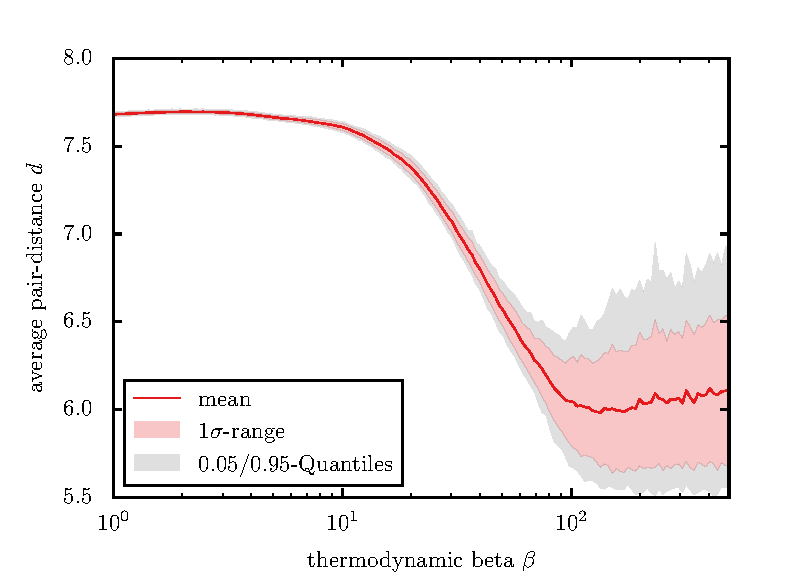
\includegraphics{./figures/temp_dep_coulomb2d.pdf}
	\caption{Temperature depedence}
\end{figure}


\section{Visualisation} \label{Sec:Visualisation}
\section{Further Analysis} \label{Sec:Further_Analysis}

\FloatBarrier
% BIBLIOGRAPHY
\vspace{\fill}
\begin{thebibliography}{9}
\bibitem{JPL}
	Jet Propulsion Laboratory,
	\emph{Small-Body Database Browser},\\
	\url{http://ssd.jpl.nasa.gov/sbdb.cgi?sstr=2004%20BL86;old=0;orb=0;cov=0;log=0;cad=0#orb} (Last access: 20. June 2015)
\end{thebibliography}
\end{document}